\documentclass[10pt,english,aspectratio=169]{beamer}
% Use notes or hide notes or show only notes or handout


\usetheme{default}

\usepackage{xstring}
\usepackage{pgfpages}
%\makeatletter
%\IfSubStr{\@classoptionslist}{handout}
%  {\pgfpagesuselayout{2 on 1}[letterpaper,border shrink=5mm]}
%  {}
%\makeatother

\usepackage{amsmath,amssymb,amsthm}
\usepackage{stmaryrd}
\usepackage{enumerate}
\usepackage{stfloats}
\usepackage{bbm}
\usepackage{pdfpages}
\usepackage{framed}
\usepackage{tabularx}
\usepackage{scalerel}

\usepackage{xr}
\externaldocument{../optimization}

\usepackage[most]{tcolorbox}
\tcbset{highlight math style={enhanced,
  colframe=white,colback=yellow!15,arc=8pt,boxrule=1pt,
  }}
  
\usepackage{tikz,pgf,pgfplots}
\usepackage{algorithm,algorithmic}
\usepgflibrary{shapes}
\usetikzlibrary{%
  arrows,%
  arrows.meta,
  backgrounds,
  shapes.misc,% wg. rounded rectangle
  shapes.arrows,%
  shapes,%
  calc,%
  chains,%
  matrix,%
  positioning,% wg. " of "
  scopes,%
  decorations.pathmorphing,% /pgf/decoration/random steps | erste Graphik
  shadows,%
  backgrounds,%
  fit,%
  petri,%
  quotes
}

\tikzset{background rectangle/.style={
    fill=white,
  },
  use background/.style={    
    show background rectangle
  }
}

\setbeamersize{text margin left=10mm,text margin right=35mm}

\pgfplotsset{compat=1.12}

%\usetheme{Frankfurt}
%\usecolortheme{ldpc}
\useinnertheme{rounded}
\usecolortheme{whale}
\usecolortheme{orchid}

\newcommand{\ul}[1]{\underline{#1}}
\renewcommand{\Pr}{\mathbb{P}}

%% Setup slides and notes
\makeatletter
\IfSubStr{\@classoptionslist}{notes} { \IfSubStr{\@classoptionslist}{hide} {}{\IfSubStr{\@classoptionslist}{only} {}{\setbeameroption{show notes on second screen=right}}} }{}
\makeatother
%\setbeamertemplate{note page}{\pagecolor{yellow!5}\vfill\insertnote\vfill}

\newcommand{\getpdfpages}[2]{\begingroup
  \setbeamercolor{background canvas}{bg=}
  \addtocounter{framenumber}{1}
  \includepdf[pages={#1},%
  pagecommand={%
    \expandafter\def\expandafter\insertshorttitle\expandafter{%
      \insertshorttitle\hfill\insertframenumber\,/\,\inserttotalframenumber}}%
  ]{#2}
  \endgroup}

\newcommand{\backupbegin}{
   \newcounter{finalframe}
   \setcounter{finalframe}{\value{framenumber}}
}
\newcommand{\backupend}{
   \setcounter{framenumber}{\value{finalframe}}
}

 \setbeamercolor{bibliography entry author}{fg=black}
 \setbeamercolor{bibliography entry title}{fg=black}
 \setbeamercolor{bibliography entry location}{fg=black}
 \setbeamercolor{bibliography entry note}{fg=black}
 
 \setbeamerfont{bibliography item}{size=\footnotesize}
 \setbeamerfont{bibliography entry author}{size=\footnotesize}
 \setbeamerfont{bibliography entry title}{size=\footnotesize}
 \setbeamerfont{bibliography entry location}{size=\footnotesize}
 \setbeamerfont{bibliography entry note}{size=\footnotesize}
 \setbeamertemplate{bibliography item}{\insertbiblabel}
 
\newlength\tikzwidth
\newlength\tikzheight


\newcommand{\mc}[1]{\mathcal{#1}}
\newcommand{\mbb}[1]{\mathbb{#1}}
%\newcommand{\expt}{\mbb{E}}
%\newcommand{\dd}{\mathrm{d}}
\newcommand{\Interior}[1]{\ensuremath{{#1}^{\circ}}}
\newcommand{\Closure}[1]{\ensuremath{\overline{#1}}}
\newcommand{\Complement}[1]{\ensuremath{{#1}^{c}}}

\newcommand{\Expect}{\ensuremath{\mathrm{E}}}
\newcommand{\vecnot}{\underline}
\newcommand{\RealNumbers}{\ensuremath{\mathbb{R}}}
\newcommand{\RationalNumbers}{\mathbb{Q}}
\newcommand{\ComplexNumbers}{\mathbb{C}}
\newcommand{\Real}{\mathrm{Re}}
\newcommand{\Span}{\mathrm{span}}
\newcommand{\Rank}{\mathrm{rank}}
\newcommand{\Nullity}{\mathrm{nullity}}
\newcommand{\Trace}{\mathrm{tr}}
\newcommand{\Diag}{\mathrm{diag}}
\newcommand{\dd}{\mathrm{d}}
\DeclareMathOperator*{\esssup}{ess\,sup}

% Use < , > inner product
\newcommand{\inner}[2]{{\left\langle #1 \mskip2mu , #2 \right\rangle}}
\newcommand{\tinner}[2]{{\langle #1 \mskip1mu , #2 \rangle}}

% Use < | > inner product
%\newcommand{\inner}[2]{{\left\langle #1 \mskip2mu \middle| \mskip2mu #2 \right\rangle}}
%\newcommand{\tinner}[2]{{\langle #1 \mskip1mu | \mskip1mu  #2 \rangle}}




\def\checkmark{\tikz\fill[scale=0.4](0,.35) -- (.25,0) -- (1,.7) -- (.25,.15) -- cycle;}
\def\greencheck{{\color{green}\checkmark}}
\def\scalecheck{\resizebox{\widthof{\checkmark}*\ratio{\widthof{x}}{\widthof{\normalsize x}}}{!}{\checkmark}}
\def\xmark{\tikz [x=1.4ex,y=1.4ex,line width=.2ex, red] \draw (0,0) -- (1,1) (0,1) -- (1,0);}
\def\redx{{\color{red}\xmark}}

\renewcommand{\footnotesep}{-2pt}


\begin{document}

\title{ECE 586: Vector Space Methods \\ Lecture 23: Constrained Optimization}
\author{Henry D. Pfister \\ Duke University}
\date{}
%\date{August 20th, 2020}
%\maketitle

\setbeamertemplate{navigation symbols}{}

\begin{frame}[plain]
	\titlepage
	
	\note{
		\vspace{8mm}
		\begin{enumerate}
			\setlength\itemsep{3mm}
			\color{red}
			\item Welcome to the 11th video lecture for ECE 586, Vector Space Methods. \\[2mm]
			Today, we'll finish our discussion of subspaces and bases and then move on to linear transforms.
		\end{enumerate}
	}
\end{frame}

\addtocounter{framenumber}{-1}
\setbeamertemplate{navigation symbols}{\textcolor{blue}{\footnotesize \insertframenumber ~/ \inserttotalframenumber}}






\begin{frame}{Unconstrained Linear Optimization}

\begin{minipage}{0.45\textwidth}
Consider the unconstrained linear optimization problem:
\[ \min_{\vecnot{x} \in \mathbb{R}^n} \vecnot{c}^T \vecnot{x} = \begin{cases} 0 & \text{if } \vecnot{c} = \vecnot{0} \\ -\infty & \text{otherwise}. \end{cases} \]  

Figure shows labeled level sets of $\vecnot{c}^T \vecnot{x}$ for $n=2$ and $\color{red} \vecnot{c}=(1,2)$.

\end{minipage}
\hfill
\begin{minipage}{0.50\textwidth}
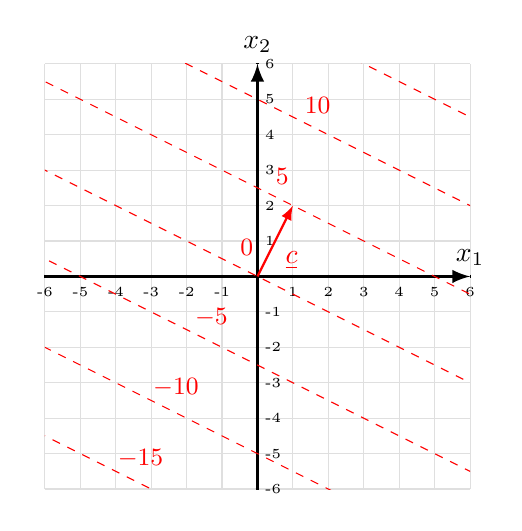
\begin{tikzpicture}[scale=0.45]

    \pgfmathtruncatemacro{\xa}{-6}
    \pgfmathtruncatemacro{\xb}{6}
    \pgfmathtruncatemacro{\ya}{-6}
    \pgfmathtruncatemacro{\yb}{6}
    \draw[gray!25, thin, step=1] (\xa,\ya) grid (\xb,\yb);
    \draw[very thick,-latex] (\xa,0) -- (\xb,0) node[above] {$x_1$};
    \draw[very thick,-latex] (0,\ya) -- (0,\yb) node[above] {$x_2$};

    \foreach \x in {\xa,...,\xb} \draw (\x,0.05) -- (\x,-0.05) node[below] {\ifthenelse{\x=0}{}{\tiny\x}};
    \foreach \y in {\ya,...,\yb} \draw (-0.05,\y) -- (0.05,\y) node[right=-0.5mm] {\ifthenelse{\y=0}{}{\tiny\y}};

    \pgfmathtruncatemacro{\vx}{1}
    \pgfmathtruncatemacro{\vy}{2}
    \draw[red,thick,-latex] (0,0) -- node[below right ,pos=0.5] {$\vecnot{c}$} (\vx,\vy);
	\begin{scope}
        \clip(\xa,\ya) rectangle (\xb,\yb);
		\foreach \i in {-4,...,4}
		    \draw[red,dashed] (\vx*\i+5*\vy,\vy*\i-5*\vx) -- node [red,pos=0.515,above=0.75mm] {\small\pgfmathparse{(\vx*\vx+\vy*\vy)*\i}\pgfmathprintnumber{\pgfmathresult}} (\vx*\i-5*\vy,\vy*\i+5*\vx);
	\end{scope}
		    
\end{tikzpicture}
\end{minipage}

\end{frame}

\begin{frame}{Constrained Linear Optimization}

\begin{minipage}{0.45\textwidth}
Now, consider the \textcolor{blue}{constrained} linear optimization problem:
\[ \min_{\vecnot{x} \in \mathcal{D}} \vecnot{c}^T \vecnot{x}. \]  

Figure shows $\color{green!40!black} \mathcal{D}$ with level sets of $\vecnot{c}^T \vecnot{x}$ for $n=2$ and $\color{red} \vecnot{c}=(1,2)$.

\vspace{3mm}

\visible<2->{ $\circ\,$~The optimal point $\color{blue} \vecnot{x}^*$ can be found using gradient descent from any initial feasible point.}

\vspace{2mm}

\visible<3->{ $\circ\,$~The \textcolor{purple!80!black}{negative gradient} is reduced by the \textcolor{green!40!black}{constraint normal} to give a \textcolor{blue}{feasible descent direction}.}

\end{minipage}
\hfill
\begin{minipage}{0.50\textwidth}
\begin{tikzpicture}[scale=0.45]
    \pgfmathtruncatemacro{\xa}{-6}
    \pgfmathtruncatemacro{\xb}{6}
    \pgfmathtruncatemacro{\ya}{-6}
    \pgfmathtruncatemacro{\yb}{6}
    \draw[gray!25, thin, step=1] (\xa,\ya) grid (\xb,\yb);
    \draw[very thick,-latex] (\xa,0) -- (\xb,0) node[above] {$x_1$};
    \draw[very thick,->] (0,\ya) -- (0,\yb) node[above] {$x_2$};

    \foreach \x in {\xa,...,\xb} \draw (\x,0.05) -- (\x,-0.05) node[below] {\ifthenelse{\x=0}{}{\tiny\x}};
    \foreach \y in {\ya,...,\yb} \draw (-0.05,\y) -- (0.05,\y) node[right=-0.5mm] {\ifthenelse{\y=0}{}{\tiny\y}};

    \pgfmathtruncatemacro{\vx}{1}
    \pgfmathtruncatemacro{\vy}{2}
    \draw[red,thick,-latex] (0,0) -- node[below right ,pos=0.5] {$\vecnot{c}$} (\vx,\vy);
	\begin{scope}
        \clip(\xa,\ya) rectangle (\xb,\yb);
		\foreach \i in {-4,...,4}
		    \draw[red,dashed] (\vx*\i+5*\vy,\vy*\i-5*\vx) -- node [red,pos=0.515,above=0.75mm] {\pgfmathparse{(\vx*\vx+\vy*\vy)*\i}\pgfmathprintnumber{\pgfmathresult}} (\vx*\i-5*\vy,\vy*\i+5*\vx);
	\end{scope}

	\fill[green!50!black,opacity=0.25] (15/3,10/3) -- (1/3,-6/3) -- (13/3,-15/3) -- cycle;
	\draw (4.2,1.5) node[green!40!black] {$\mathcal{D}$};
	\only<2->{%
	  \draw (13/3,-15/3) node[circle,fill=blue,inner sep=1pt,node contents={}];
	  \draw (13/3,-15/3) node[below,blue] {$\vecnot{x}^*$};
	}
    \only<3->{%
      \draw[purple!80!black,thick,-latex] (3,-4) -- (3-\vx/2,-4-\vy/2);
      \draw[green!40!black,thick,->] (3,-4) -- (3+3/5,-4+3/4);
      \draw[blue,thick,-latex] (3,-4) -- (3+2/3,-4-2/4);
    }
		
\end{tikzpicture}
\end{minipage}

\end{frame}

\begin{frame}{Linear Programs}

The optimization of a linear function with arbitrary affine equality and \\ inequality constraints is called a \textcolor{blue}{linear program (LP)}.

\vspace{3mm}

LPs have many equivalent forms because:
\begin{itemize}

\item $x_1 \!=\! 0$ is the same as $(x_1 \leq 0) \wedge (x_1\geq 0)$
\item $x_1 \leq 0$ is the same as $(x_1 + x_2 = 0) \wedge (x_2 \geq 0)$ for slack variable $x_2$
\item $x_1$ free is the same as $x_1 = x_2 - x_3$ with slack vars $x_2 \geq 0$ and $x_3 \geq 0$
\item negation swaps: $\min \leftrightarrow \max$ for objective and $\geq \,\leftrightarrow\, \leq$ for constraints
\end{itemize}  

\begin{definition}
Any LP can be transformed into one of the standard $\min$ forms: \\[1mm]
\hrule \vspace{0mm}
\begin{minipage}{0.49\textwidth}
\vspace{-2mm}
\begin{align*}
\mathrm{minimize} \quad & \vecnot{c}^T \vecnot{x} \\
\mathrm{subject\,to} \quad & A \vecnot{x} = \vecnot{b} \\
& \vecnot{x} \succeq \vecnot{0}
\end{align*}
\end{minipage}
\vrule
\begin{minipage}{0.49\textwidth}
\vspace{-2mm}
\begin{align*}
\mathrm{minimize} \quad & \vecnot{c}^T \vecnot{x} \\
\mathrm{subject\,to} \quad & A \vecnot{x} \succeq \vecnot{b} \\
& \vecnot{x} \succeq \vecnot{0}
\end{align*}
\end{minipage}
\end{definition}

\end{frame}


\begin{frame}{Duality in Linear Programs}

\uncover<1->{Let $p^*$ be the value of the linear program:
\begin{align*}
\mathrm{minimize} \quad & \textcolor{red}{x_{1}+2x_{2}} \\
\mathrm{subject\,to} \quad & 18 x_{1} + 25 x_{2} \geq -47\\
& 96 x_{1} - 87 x_{2} \geq 190\\
& -75 x_{1} + 6 x_{2} \geq -355\\
\end{align*}}

\vspace{-9mm}

\uncover<2->{\textcolor{blue}{Since $(x_1,x_2) = (4,-4)$ satisfies the constraints}, we know \textcolor{red}{$p^* \leq 4 - 8 = -4$.}}

\vspace{4mm}

\uncover<3->{One can lower bound $p^*$ by finding a \textcolor{blue}{positive linear combination of the constraints that equals the objective}.}

\vspace{2mm}

\uncover<4->{Combining the constraints with coefs $(\lambda_1,\lambda_2,\lambda_3) = \left(\frac{52}{661},0,\frac{11}{1983}\right)$ gives \vspace{-2mm}
\[ \textcolor{red}{x_1 + 2 x_2} \geq -\tfrac{17}{3} \approx -5.66. \]
}

\vspace{-4mm}

\uncover<5->{In essence, this is how \textcolor{blue}{Lagrangian duality} works and implies \textcolor{red}{$p^* \geq -5.66$}.}

\end{frame}


\iffalse
\begin{frame}{Duality in Linear Programs}

\uncover<1->{Let $p^*$ be the value of the linear program:
\begin{align*}
\mathrm{minimize} \quad & \textcolor{red}{3x_{1}-x_{2}+2x_{3}} \\
\mathrm{subject\,to} \quad & 2x_{1}-x_{2}+x_{3} \geq-1\\
& x_{1}+ 0 x_{2} + 2x_{3} \geq2\\
& -7x_{1}+4x_{2}-6x_{3} \geq1\\
\end{align*}}

\vspace{-9mm}

\uncover<2->{\textcolor{blue}{Since $(x_1,x_2,x_3) = (0,2,1)$ satisfies the constraints with value 0}, \textcolor{red}{$p^* \leq 0$.}}

\vspace{4mm}

\uncover<3->{One can \textcolor{blue}{lower bound $p^*$ by finding a linear combination of the constraints} that equals (or bounds) the objective.}

\vspace{2mm}

\uncover<4->{Combining the constraints with coefs $(\lambda_1,\lambda_2,\lambda_3) = (2,0.75,0.25)$ gives \vspace{-2mm}
\[ \textcolor{red}{3 x_1 - x_2 + 2 x_3} \geq -0.25. \]
}

\vspace{-4mm}

\uncover<5->{In essence, this is how \textcolor{blue}{Lagrangian duality} works and implies \textcolor{red}{$p^* \geq -0.25$}.}

\end{frame}
\fi


%\begin{frame}{5.4: Constrained Non-Linear Optimization}

\begin{frame}{{\ref{sec:constrained_optimization}}: Constrained Non-Linear Optimization}

\iffalse
Lagrangian optimization is an indispensable tool in engineering and physics that allows one to solve constrained non-linear optimization problems.
\fi

Consider a constrained non-linear optimization problem over $\mathcal{D} \subseteq \mathbb{R}^n$  in the following \textcolor{blue}{standard form}.
Let $f_i \colon \mathcal{D} \rightarrow \mathbb{R}$ and $h_j \colon \mathcal{D} \rightarrow \mathbb{R}$ be real functionals for $i=0,1,\ldots,m$ and $j=1,2,\ldots,p$.
Then, we write
\begin{align*}
\mathrm{minimize} \quad & f_0 (\vecnot{x}) \\
\mathrm{subject\,to} \quad & f_i (\vecnot{x}) \leq 0, \quad i=1,2,\ldots,m \\
& h_j (\vecnot{x}) = 0, \quad j=1,2,\ldots,p.
\end{align*}

\hrule

\begin{itemize}
\item<2-> the function $f_0$ is called the \textcolor{blue}{objective function}
\item<3-> the functions $f_1,\ldots,f_m$ define \textcolor{blue}{inequality constraints}
\item<4-> the functions $h_1,\ldots,h_p$ define \textcolor{blue}{equality constraints}
\item<5-> \textcolor{blue}{feasible} points in $\mathcal{F} \triangleq \{ \vecnot{x}\in \mathcal{D} \, | \,  f_i (\vecnot{x}) \leq 0, i\in [m], h_j (\vecnot{x}) = 0, j\in[p] \}$ satisfy all constraints and the problem is feasible if $\mathcal{F} \neq \emptyset$.
\item<6-> the \textcolor{blue}{optimal value} is $p^* \triangleq \inf \left\{ f_0 (\vecnot{x}) \, | \, \vecnot{x} \in \mathcal{F} \right\}$
\item<7-> problem called \textcolor{blue}{convex} if all $f_i$ convex and all $h_j$ affine: $h_j (\vecnot{x}) \!=\! \vecnot{a}_j^T \vecnot{x} \!-\! b_j \!\!\!$ 
\end{itemize}

\end{frame}

\begin{frame}{General Example}

\vspace{-2mm}

  \begin{center}
    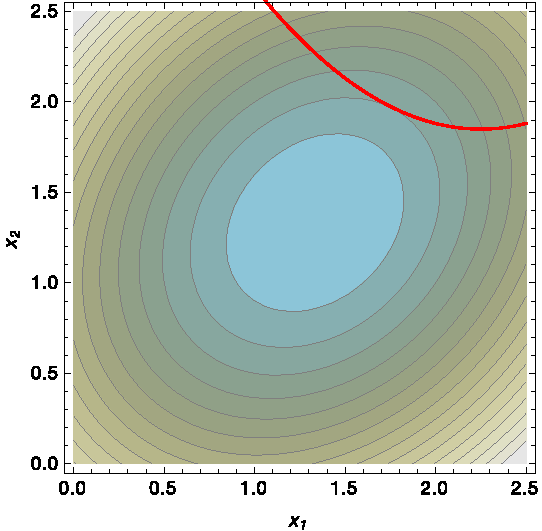
\includegraphics[width=65mm]{opt_fig}
  \end{center}

\vspace{-2mm}

Contour plot of $f_0 (x_1,x_2) = (x_1 - 1)^2 + (x_2 - 1)^2 - x_1 x_2 /2$ whose minimum occurs at $(4/3,4/3)$ (i.e., center of blue ellipse).  The red line shows the inequality constraint $f_1 (x_1,x_2)= 1.85 + (x_1 - 2.25)^2 / 2 - x_2 \leq 0$

\end{frame}



\begin{frame}{Langrangian Formulation}

Used to transform from constrained to unconstrained optimization

\begin{definition}
For the standard optimization, the \textcolor{blue}{Lagrangian} $L \colon \mathcal{D} \times \mathbb{R}^m \times \mathbb{R}^p \rightarrow \mathbb{R}$ is \vspace{-2mm}
\[ L(\vecnot{x},\vecnot{\lambda},\vecnot{\nu}) = f_0(\vecnot{x}) + \sum_{i=1}^m \lambda_i f_i(\vecnot{x}) + \sum_{j=1}^p \nu_j h_j(\vecnot{x}), \vspace{-1.5mm} \]
where the \textcolor{blue}{Lagrange multipliers} $\lambda_i$ and $\nu_j$ define penalties associated with violating the $i$-th inequality and $j$-th equality constraints, respectively.
\end{definition}

\begin{theorem}[{\ref{theorem:KKT}}) (Karush-Kuhn-Tucker]<2->
If $\vecnot{x}^*$ is a constrained local optimum that satisfies a constraint qualification (e.g., mild technical conditions) and $A = \{ i\in [m] \, | \, f_i (\vecnot{x}^*)=0 \}$ is the set of active constraints at $\vecnot{x}^*$, then there exist $\vecnot{\lambda}^* \geq 0$ and $\vecnot{\nu}^*$ such that
\vspace{-2mm}
\begin{align*}
\nabla_\vecnot{x} L(\vecnot{x},\vecnot{\lambda},\vecnot{\nu}) = \nabla f_0 (\vecnot{x}^*) + \sum_{i\in A} \lambda_i^* \nabla f_i (\vecnot{x}^*) + \sum_{j=1}^p \nu_j^* \nabla h_j (\vecnot{x}^*) &= \vecnot{0}. \vspace{-1mm}
\end{align*}
\end{theorem}

% Add example pic with vector additions

\end{frame}

\iffalse
\begin{frame}{Lagrangian Example}

For the pictured example, the Lagrangian is given by
\[ L(\vecnot{x},\lambda) = \underbrace{(x_1 \!-\! 1)^2 + (x_2 \!-\! 1)^2 - \frac{x_1 x_2}{2}}_{f_0(\vecnot{x})} + \lambda \Bigg( \underbrace{1.85 + \frac{(x_1 - 2.25)^2}{2} \!-\! x_2}_{f_1 (\vecnot{x})} \Bigg) \]

\centering
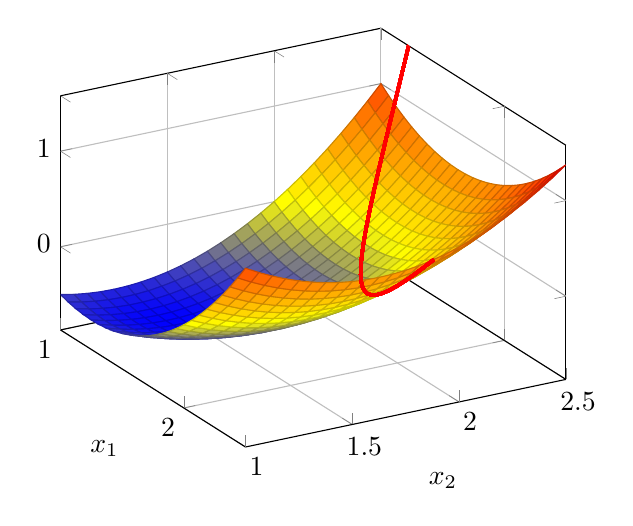
\begin{tikzpicture}
  \begin{axis}[width=80mm,view={60}{30},grid=major,ymin=1.0,ymax=2.5,xmin=1.0,xmax=2.5,xlabel=$x_1$,ylabel=$x_2$]
    \addplot3 [surf,domain=1:2.5] {(x-1)^2 + (y-1)^2 - x*y/2 + 0*(1.85+(x-2.25)^2/2-y)};
    %\addlegendentry{$\lambda=0$}
    
    %\addplot3 [surf,domain=1:2.5] {(x-1)^2 + (y-1)^2 - x*y/2 + 1*(1.85+(x-2.25)^2/2-y)};
    %\addlegendentry{$\lambda=1$}

    \addplot3 [variable=x,mesh,domain=1.0:2.5,red,very thick] ({x},{(1.85+((x-2.25)^2)/2)},{(x-1)^2 + ((1.85+((x-2.25)^2)/2)-1)^2 - x*(1.85+((x-2.25)^2)/2)/2});
    %\addlegendentry{$constraint$}
\end{axis}
\end{tikzpicture}
\end{frame}


\fi

\begin{frame}{Langrangian Duality}

\begin{definition}
The \textcolor{blue}{Lagrangian dual function} is defined to be \vspace{-1.5mm}
\[ g(\vecnot{\lambda},\vecnot{\nu}) \triangleq \inf_{\vecnot{x}\in \mathcal{D}} L(\vecnot{x},\vecnot{\lambda},\vecnot{\nu}) = \inf_{\vecnot{x}\in \mathcal{D}} \Bigg( f_0(\vecnot{x}) + \sum_{i=1}^m \lambda_i f_i(\vecnot{x}) + \sum_{j=1}^p \nu_j h_j(\vecnot{x}) \Bigg). \]
\end{definition}


%The pointwise infimum of linear functions is concave because
%\[ \inf_{\vecnot{x}\in \mathcal{D}} %L(\vecnot{x},\vecnot{\lambda},\vecnot{\nu})  \inf]

\begin{lemma}<2->
The Lagrangian dual function is concave and the \textcolor{blue}{Lagrangian dual problem}, \vspace{-2.5mm}
\begin{align*}
\mathrm{maximize} \quad & g(\vecnot{\lambda},\vecnot{\nu}) \\
\mathrm{subject\,to} \quad & \vecnot{\lambda} \geq 0, \vspace{-1mm}
\end{align*}
has a unique max value $d^* \leq p^*$.
This property is known as \textcolor{blue}{weak duality}.
\end{lemma}

\begin{definition}<3->
If $d^* = p^*$, then one says that \textcolor{blue}{strong duality} holds for the problem.
\end{definition}

%\visible<3->{Proof of lemma on whiteboard}

\end{frame}

\begin{frame}{Weak Duality Proof}
\part{title}
Lagrangian dual is concave because \textcolor{blue}{pointwise infimum of affine functions}:\vspace{-1mm}
\begin{align*}
g(\alpha\vecnot{\lambda}+&(1-\alpha)\vecnot{\lambda}',\alpha\vecnot{\nu}+(1-\alpha)\vecnot{\nu}') \\
&= \inf_{\vecnot{x}\in \mathcal{D}} L(\vecnot{x},\alpha\vecnot{\lambda}+(1-\alpha)\vecnot{\lambda}',\alpha\vecnot{\nu}+(1-\alpha) \vecnot{\nu}') \\
&= \inf_{\vecnot{x}\in \mathcal{D}} \big( \alpha L(\vecnot{x},\vecnot{\lambda},\vecnot{\nu}) + (1-\alpha) L(\vecnot{x},\vecnot{\lambda}',\vecnot{\nu}') \big) \\
&\geq \inf_{\vecnot{x}\in \mathcal{D}} \alpha L(\vecnot{x},\vecnot{\lambda},\vecnot{\nu}) + \inf_{\vecnot{x}'\in \mathcal{D}} (1-\alpha) L(\vecnot{x}',\vecnot{\lambda}',\vecnot{\nu}') \\
&= \alpha g(\vecnot{\lambda},\vecnot{\nu}) + (1-\alpha) g(\vecnot{\lambda}',\vecnot{\nu}'). \vspace{-1mm}
\end{align*}
Concavity implies unique maximum value $d^*$ upper bounded by \vspace{-2mm}
\begin{align*}
g(\vecnot{\lambda},\vecnot{\nu})
&= \inf_{\vecnot{x}\in \mathcal{D}} L(\vecnot{x},\vecnot{\lambda},\vecnot{\nu})
\stackrel{(a)}{\leq} \inf_{\vecnot{x}\in \mathcal{F}} L(\vecnot{x},\vecnot{\lambda},\vecnot{\nu}) \\
&\stackrel{(b)}{=} p^* + \sum_{i=1}^m \lambda_i f_i (\vecnot{x})
\stackrel{(c)}{\leq} p^*, \vspace{-3mm}
\end{align*}
where $(a)$ is implied by $\mathcal{F} \subseteq \mathcal{D}$, $(b)$ follows from $h_j(\vecnot{x}) = 0$ for $\vecnot{x}\in \mathcal{F}$, and $(c)$ holds by combining $f_i(\vecnot{x}) \leq 0$ for $\vecnot{x}\in \mathcal{F}$ and $\lambda_i \geq 0$.

\end{frame}

\begin{frame} \frametitle{The Lagrangian Dual Problem}

While $g(\vecnot{\lambda},\vecnot{\nu})$ can be $-\infty$, this is avoided by defining the \textcolor{blue}{dual feasible set}:
\begin{align*}
\mathcal{C} &\triangleq \left\{ (\vecnot{\lambda},\vecnot{\nu}) \in \mathbb{R}^m \times \mathbb{R}^p \,|\, \vecnot{\lambda}\succeq \vecnot{0},  g(\vecnot{\lambda},\vecnot{\nu}) > -\infty \right\}.
\end{align*}
The value of the dual optimization problem is \vspace{-1mm}
\[ d^* = \sup_{(\vecnot{\lambda},\vecnot{\nu})\in \mathcal{C}} g(\vecnot{\lambda},\vecnot{\nu}). \vspace{-1mm} \]
If $\mathcal{C} \neq \emptyset$, then the dual problem is feasible and, by definition, $d^* > -\infty$.

\vspace{6mm}

Consider the LP defined by \vspace{-2mm}
\begin{align*}
\mathrm{minimize} \quad & \vecnot{c}^T \vecnot{x} \\
\mathrm{subject\,to} \quad & A \vecnot{x} = \vecnot{b} \\
& \vecnot{x} \succeq \vecnot{0}.
\end{align*}

\end{frame}

\begin{frame} \frametitle{Lagrangian Duality for Linear Programs}

For the previous LP, the Lagrangian is given by
	\[ L(\vecnot{x},\vecnot{\lambda},\vecnot{\nu}) = \vecnot{c}^T \vecnot{x} + \vecnot{\nu}^T (\vecnot{b} - A\vecnot{x}) - \vecnot{\lambda}^T \vecnot{x}, \]
	where $-\vecnot{\lambda}^T \vecnot{x}$ corresponds to $\vecnot{x} \succeq \vecnot{0}$ and the Lagrangian dual function is \vspace{-1.5mm}
\begin{equation*}
g(\vecnot{\lambda},\vecnot{\nu})
= \inf_{\vecnot{x}\in \mathcal{D}} L(\vecnot{x},\vecnot{\lambda},\vecnot{\nu})
	= \begin{cases} \vecnot{b}^T \vecnot{\nu} & \text{if } \vecnot{c} - A^T \vecnot{\nu} - \vecnot{\lambda} = \vecnot{0} \\
-\infty & \text{otherwise}. \end{cases}
\end{equation*}
Adding the implied constraint and using $\vecnot{\lambda} \succeq \vecnot{0}$, one gets the dual LP problem
\begin{align*}
\mathrm{maximize} \quad & \vecnot{b}^T \vecnot{\nu} \\
	\mathrm{subject\,to} \quad & A^T \vecnot{\nu} \preceq \vecnot{c}.
\end{align*}

\vspace{1mm}
Strong duality for linear programs says that, if the original LP has an optimal solution (i.e., it is neither unbounded nor infeasible), then the dual LP has an optimal solution of the same value.

\end{frame}

\begin{frame} \frametitle{Next Steps}

\begin{itemize}
\setlength\itemsep{5mm}
\item To continue studying after this video -- \vspace{2mm}

\begin{itemize}
 \setlength\itemsep{3mm}
 
 \item Try the required reading:  Course Notes EF 5.4 - 5.4.3

 \item Also, look at the problems in Assignment 9
\end{itemize}
\end{itemize}

\note{
	\vspace{8mm}
	\begin{enumerate}
		\setlength\itemsep{3mm}
		\color{red}
		\item Here are some options to continue learning this material. (read) \\ [2mm]  That's it for today.  So, I'll see you next time.
	\end{enumerate}
}

\end{frame}

\end{document}



\backupbegin

%\begin{frame}
%\frametitle{Backup Slides}
%\begin{itemize}
%\item Slide numbers not included in denominator!
%\end{itemize}
%\end{frame}

%\begin{frame}[allowframebreaks]
%\frametitle{References}
%\bibliographystyle{alpha}
%\footnotesize
%\bibliography{IEEEabrv,WCLabrv,WCLbib,WCLnewbib}
%\end{frame}

\backupend

\end{document}
